\documentclass[8pt,aspectratio=169]{beamer}
\usetheme{Madrid}
\usepackage{graphicx}
\usepackage{booktabs}
\usepackage{adjustbox}
\usepackage{multicol}
\usepackage{amsmath}
\usepackage{amssymb}
\usepackage{listings}
\usepackage{xcolor}

% Color definitions
\definecolor{mlblue}{RGB}{0,102,204}
\definecolor{mlpurple}{RGB}{51,51,178}
\definecolor{mllavender}{RGB}{173,173,224}
\definecolor{mllavender2}{RGB}{193,193,232}
\definecolor{mllavender3}{RGB}{204,204,235}
\definecolor{mllavender4}{RGB}{214,214,239}
\definecolor{mlorange}{RGB}{255, 127, 14}
\definecolor{mlgreen}{RGB}{44, 160, 44}
\definecolor{mlred}{RGB}{214, 39, 40}
\definecolor{mlgray}{RGB}{127, 127, 127}

% Additional colors for template compatibility
\definecolor{lightgray}{RGB}{240, 240, 240}
\definecolor{midgray}{RGB}{180, 180, 180}

% Solidity colors
\definecolor{solkeyword}{RGB}{0,102,153}
\definecolor{solstring}{RGB}{163,21,21}
\definecolor{solcomment}{RGB}{0,128,0}
\definecolor{solnumber}{RGB}{0,128,128}

% Solidity language definition
\lstdefinelanguage{Solidity}{
  keywords={pragma, solidity, contract, function, public, private, external, internal, view, pure, payable, returns, return, if, else, for, while, mapping, address, uint, uint256, int, string, bool, bytes, bytes32, event, emit, modifier, require, constructor, memory, storage, calldata, msg, sender, value, this, new, delete, true, false},
  keywordstyle=\color{solkeyword}\bfseries,
  sensitive=true,
  comment=[l]{//},
  morecomment=[s]{/*}{*/},
  commentstyle=\color{solcomment}\ttfamily,
  stringstyle=\color{solstring}\ttfamily,
  morestring=[b]',
  morestring=[b]"
}

% Apply custom colors to Madrid theme
\setbeamercolor{palette primary}{bg=mllavender3,fg=mlpurple}
\setbeamercolor{palette secondary}{bg=mllavender2,fg=mlpurple}
\setbeamercolor{palette tertiary}{bg=mllavender,fg=white}
\setbeamercolor{palette quaternary}{bg=mlpurple,fg=white}
\setbeamercolor{structure}{fg=mlpurple}
\setbeamercolor{section in toc}{fg=mlpurple}
\setbeamercolor{subsection in toc}{fg=mlblue}
\setbeamercolor{title}{fg=mlpurple}
\setbeamercolor{frametitle}{fg=mlpurple,bg=mllavender3}
\setbeamercolor{block title}{bg=mllavender2,fg=mlpurple}
\setbeamercolor{block body}{bg=mllavender4,fg=black}

\setbeamertemplate{navigation symbols}{}
\setbeamertemplate{itemize items}[circle]
\setbeamertemplate{enumerate items}[default]
\setbeamersize{text margin left=5mm,text margin right=5mm}

\newcommand{\bottomnote}[1]{%
\vfill
\vspace{-2mm}
\textcolor{mllavender2}{\rule{\textwidth}{0.4pt}}
\vspace{1mm}
\footnotesize
\textbf{#1}
}

% TikZ and pgfplots packages
\usepackage{tikz}
\usepackage{pgfplots}
\pgfplotsset{compat=1.18}
\usetikzlibrary{arrows.meta, positioning, shapes.geometric, shapes.symbols, calc, decorations.pathmorphing, mindmap}

\title{Crypto Trading \& Markets: A Visual Introduction}
\subtitle{Standalone Mini-Lecture}
\author{Prof.~Dr.~Joerg Osterrieder}
\institute{University Lecture Series}
\date{\today}
\begin{document}

% ==================== FRAME 1: TITLE ====================
\begin{frame}[plain]
\vspace{2cm}
\begin{center}
{\Huge\color{mlpurple} Crypto Trading \& Markets: A Visual Introduction}\\[0.4cm]
{\Large\color{mlblue} Standalone Mini-Lecture}\\[0.3cm]
\textcolor{mlgray}{\rule{6cm}{0.4pt}}\\[0.3cm]
{\small\itshape ``Markets can remain irrational longer than you can remain solvent'' -- John Maynard Keynes}\\[1.5cm]
{\normalsize Prof.~Dr.~Joerg Osterrieder}\\[0.2cm]
{\small University Lecture Series}\\[0.2cm]
{\small \today}
\end{center}

\bottomnote{This mini-lecture covers how crypto exchanges work, order books, trading strategies, risk metrics, and market structure.}
\end{frame}

% ==================== FRAME 2: HOW DO CRYPTO EXCHANGES WORK? ====================
\begin{frame}{How Do Crypto Exchanges Work?}
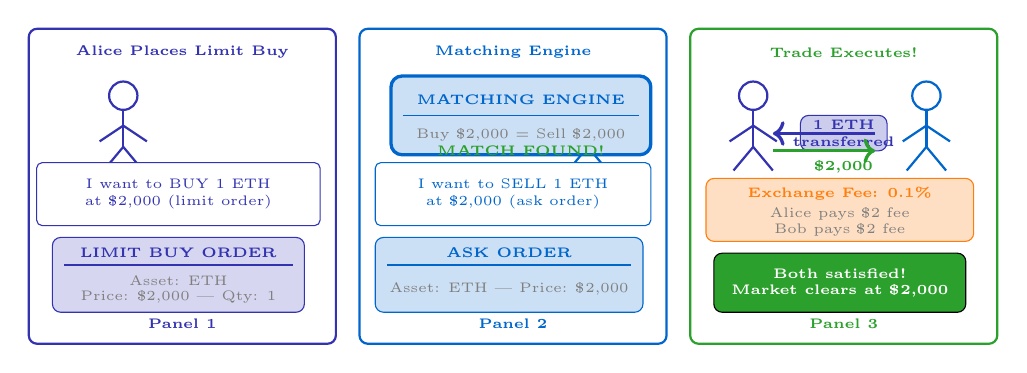
\begin{tikzpicture}
  % Panel borders
  \draw[thick, mlpurple, rounded corners=3pt] (0.1,0.2) rectangle (4.0,4.2);
  \draw[thick, mlblue,   rounded corners=3pt] (4.3,0.2) rectangle (8.2,4.2);
  \draw[thick, mlgreen,  rounded corners=3pt] (8.5,0.2) rectangle (12.4,4.2);

  % --- Panel 1: Alice places limit buy ---
  \node[font=\tiny\bfseries, mlpurple] at (2.05,3.9) {Alice Places Limit Buy};
  % Alice stick figure
  \draw[mlpurple,thick] (1.3,3.35) circle (0.18);
  \draw[mlpurple,thick] (1.3,3.17) -- (1.3,2.70);
  \draw[mlpurple,thick] (1.3,2.97) -- (1.0,2.77);
  \draw[mlpurple,thick] (1.3,2.97) -- (1.6,2.77);
  \draw[mlpurple,thick] (1.3,2.70) -- (1.05,2.40);
  \draw[mlpurple,thick] (1.3,2.70) -- (1.55,2.40);
  % Speech bubble from Alice
  \draw[fill=white, draw=mlpurple, rounded corners=2pt] (0.2,1.7) rectangle (3.8,2.5);
  \node[font=\tiny, mlpurple, align=center] at (2.0,2.1) {I want to BUY 1 ETH\\at \$2{,}000 (limit order)};
  % Order ticket box
  \draw[fill=mlpurple!20, draw=mlpurple, rounded corners=3pt] (0.4,0.6) rectangle (3.6,1.55);
  \node[font=\tiny\bfseries, mlpurple, align=center] at (2.0,1.35) {LIMIT BUY ORDER};
  \draw[mlpurple, thin] (0.55,1.2) -- (3.45,1.2);
  \node[font=\tiny, mlgray, align=center] at (2.0,1.0) {Asset: ETH};
  \node[font=\tiny, mlgray, align=center] at (2.0,0.8) {Price: \$2{,}000 | Qty: 1};
  \node[font=\tiny\bfseries, mlpurple] at (2.05,0.45) {Panel 1};

  % --- Panel 2: Matching engine connects them ---
  \node[font=\tiny\bfseries, mlblue] at (6.25,3.9) {Matching Engine};
  % Bob stick figure
  \draw[mlblue,thick] (7.2,3.35) circle (0.18);
  \draw[mlblue,thick] (7.2,3.17) -- (7.2,2.70);
  \draw[mlblue,thick] (7.2,2.97) -- (6.9,2.77);
  \draw[mlblue,thick] (7.2,2.97) -- (7.5,2.77);
  \draw[mlblue,thick] (7.2,2.70) -- (6.95,2.40);
  \draw[mlblue,thick] (7.2,2.70) -- (7.45,2.40);
  % Speech bubble from Bob
  \draw[fill=white, draw=mlblue, rounded corners=2pt] (4.5,1.7) rectangle (8.0,2.5);
  \node[font=\tiny, mlblue, align=center] at (6.25,2.1) {I want to SELL 1 ETH\\at \$2{,}000 (ask order)};
  % Matching engine box in center
  \draw[fill=mlblue!20, draw=mlblue, very thick, rounded corners=4pt] (4.7,2.6) rectangle (8.0,3.6);
  \node[font=\tiny\bfseries, mlblue, align=center] at (6.35,3.3) {MATCHING ENGINE};
  \draw[mlblue, thin] (4.85,3.1) -- (7.85,3.1);
  \node[font=\tiny, mlgray, align=center] at (6.35,2.85) {Buy \$2{,}000 = Sell \$2{,}000};
  \node[font=\tiny\bfseries, mlgreen, align=center] at (6.35,2.65) {MATCH FOUND!};
  % Order ticket box
  \draw[fill=mlblue!20, draw=mlblue, rounded corners=3pt] (4.5,0.6) rectangle (7.9,1.55);
  \node[font=\tiny\bfseries, mlblue, align=center] at (6.2,1.35) {ASK ORDER};
  \draw[mlblue, thin] (4.65,1.2) -- (7.75,1.2);
  \node[font=\tiny, mlgray, align=center] at (6.2,0.9) {Asset: ETH | Price: \$2{,}000};
  \node[font=\tiny\bfseries, mlblue] at (6.25,0.45) {Panel 2};

  % --- Panel 3: Trade executes ---
  \node[font=\tiny\bfseries, mlgreen] at (10.45,3.9) {Trade Executes!};
  % Alice happy
  \draw[mlpurple,thick] (9.3,3.35) circle (0.18);
  \draw[mlpurple,thick] (9.3,3.17) -- (9.3,2.70);
  \draw[mlpurple,thick] (9.3,2.97) -- (9.0,2.77);
  \draw[mlpurple,thick] (9.3,2.97) -- (9.6,2.77);
  \draw[mlpurple,thick] (9.3,2.70) -- (9.05,2.40);
  \draw[mlpurple,thick] (9.3,2.70) -- (9.55,2.40);
  % Bob happy
  \draw[mlblue,thick] (11.5,3.35) circle (0.18);
  \draw[mlblue,thick] (11.5,3.17) -- (11.5,2.70);
  \draw[mlblue,thick] (11.5,2.97) -- (11.2,2.77);
  \draw[mlblue,thick] (11.5,2.97) -- (11.8,2.77);
  \draw[mlblue,thick] (11.5,2.70) -- (11.25,2.40);
  \draw[mlblue,thick] (11.5,2.70) -- (11.75,2.40);
  % ETH token exchanged
  \draw[fill=mlpurple!25, draw=mlpurple, rounded corners=3pt] (9.9,2.65) rectangle (11.0,3.1);
  \node[font=\tiny\bfseries, mlpurple, align=center] at (10.45,2.87) {1 ETH\\transferred};
  % Arrow from Bob to Alice
  \draw[->, very thick, mlpurple] (10.85,2.87) -- (9.55,2.87);
  % USD arrow from Alice to Bob
  \draw[->, very thick, mlgreen] (9.55,2.65) -- (10.85,2.65);
  \node[font=\tiny\bfseries, mlgreen, align=center] at (10.45,2.45) {\$2{,}000};
  % Fee box
  \draw[fill=mlorange!25, draw=mlorange, rounded corners=3pt] (8.7,1.5) rectangle (12.1,2.3);
  \node[font=\tiny\bfseries, mlorange, align=center] at (10.4,2.1) {Exchange Fee: 0.1\%};
  \node[font=\tiny, mlgray, align=center] at (10.4,1.75) {Alice pays \$2 fee\\Bob pays \$2 fee};
  % Happy result
  \draw[fill=mlgreen, rounded corners=3pt] (8.8,0.6) rectangle (12.0,1.35);
  \node[font=\tiny\bfseries, white, align=center] at (10.4,0.97) {Both satisfied!\\Market clears at \$2{,}000};
  \node[font=\tiny\bfseries, mlgreen] at (10.45,0.45) {Panel 3};
\end{tikzpicture}

\bottomnote{A crypto exchange's matching engine connects buyers and sellers automatically, executing trades when bid and ask prices meet.}
\end{frame}

% ==================== FRAME 3: THE ORDER BOOK ====================
\begin{frame}{The Order Book}
\begin{columns}[c]
  \begin{column}{0.52\textwidth}
    \centering
    {\small\bfseries\color{mlpurple} Live Order Book: ETH/USD}\\[0.2cm]
    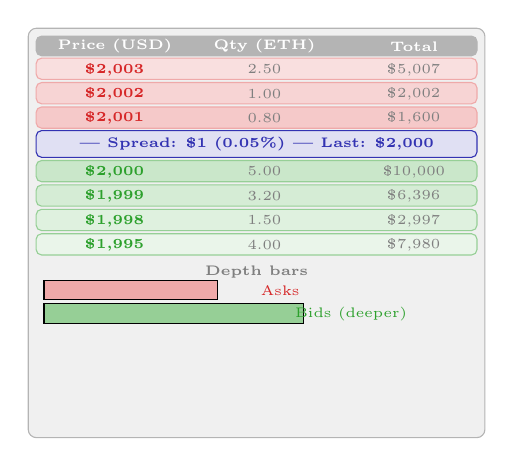
\begin{tikzpicture}
      % Background
      \draw[fill=lightgray, draw=midgray, rounded corners=3pt] (0,0) rectangle (5.8,5.2);

      % Header row
      \draw[fill=midgray, draw=midgray, rounded corners=2pt] (0.1,4.85) rectangle (5.7,5.1);
      \node[font=\tiny\bfseries, white] at (1.1,4.97) {Price (USD)};
      \node[font=\tiny\bfseries, white] at (3.0,4.97) {Qty (ETH)};
      \node[font=\tiny\bfseries, white] at (4.9,4.97) {Total};

      % ASK side (red) - above mid price
      \draw[fill=mlred!15, draw=mlred!40, rounded corners=2pt] (0.1,4.55) rectangle (5.7,4.82);
      \node[font=\tiny\bfseries, mlred] at (1.1,4.68) {\$2{,}003};
      \node[font=\tiny, mlgray] at (3.0,4.68) {2.50};
      \node[font=\tiny, mlgray] at (4.9,4.68) {\$5{,}007};

      \draw[fill=mlred!20, draw=mlred!40, rounded corners=2pt] (0.1,4.24) rectangle (5.7,4.51);
      \node[font=\tiny\bfseries, mlred] at (1.1,4.37) {\$2{,}002};
      \node[font=\tiny, mlgray] at (3.0,4.37) {1.00};
      \node[font=\tiny, mlgray] at (4.9,4.37) {\$2{,}002};

      \draw[fill=mlred!25, draw=mlred!40, rounded corners=2pt] (0.1,3.93) rectangle (5.7,4.20);
      \node[font=\tiny\bfseries, mlred] at (1.1,4.06) {\$2{,}001};
      \node[font=\tiny, mlgray] at (3.0,4.06) {0.80};
      \node[font=\tiny, mlgray] at (4.9,4.06) {\$1{,}600};

      % Spread indicator
      \draw[fill=mlpurple!15, draw=mlpurple, rounded corners=2pt] (0.1,3.56) rectangle (5.7,3.90);
      \node[font=\tiny\bfseries, mlpurple, align=center] at (2.9,3.73) {--- Spread: \$1 (0.05\%) --- Last: \$2{,}000};

      % BID side (green) - below mid price
      \draw[fill=mlgreen!25, draw=mlgreen!50, rounded corners=2pt] (0.1,3.25) rectangle (5.7,3.52);
      \node[font=\tiny\bfseries, mlgreen] at (1.1,3.38) {\$2{,}000};
      \node[font=\tiny, mlgray] at (3.0,3.38) {5.00};
      \node[font=\tiny, mlgray] at (4.9,3.38) {\$10{,}000};

      \draw[fill=mlgreen!20, draw=mlgreen!50, rounded corners=2pt] (0.1,2.94) rectangle (5.7,3.21);
      \node[font=\tiny\bfseries, mlgreen] at (1.1,3.07) {\$1{,}999};
      \node[font=\tiny, mlgray] at (3.0,3.07) {3.20};
      \node[font=\tiny, mlgray] at (4.9,3.07) {\$6{,}396};

      \draw[fill=mlgreen!15, draw=mlgreen!50, rounded corners=2pt] (0.1,2.63) rectangle (5.7,2.90);
      \node[font=\tiny\bfseries, mlgreen] at (1.1,2.76) {\$1{,}998};
      \node[font=\tiny, mlgray] at (3.0,2.76) {1.50};
      \node[font=\tiny, mlgray] at (4.9,2.76) {\$2{,}997};

      \draw[fill=mlgreen!10, draw=mlgreen!50, rounded corners=2pt] (0.1,2.32) rectangle (5.7,2.59);
      \node[font=\tiny\bfseries, mlgreen] at (1.1,2.45) {\$1{,}995};
      \node[font=\tiny, mlgray] at (3.0,2.45) {4.00};
      \node[font=\tiny, mlgray] at (4.9,2.45) {\$7{,}980};

      % Depth bar visualization
      \node[font=\tiny\bfseries, mlgray, align=center] at (2.9,2.1) {Depth bars};
      \draw[fill=mlred!40]   (0.2,1.75) rectangle (2.4,2.0);
      \draw[fill=mlgreen!50] (0.2,1.45) rectangle (3.5,1.70);
      \node[font=\tiny, mlred]   at (3.2,1.87) {Asks};
      \node[font=\tiny, mlgreen] at (4.1,1.57) {Bids (deeper)};

      % Labels
      \node[font=\tiny\bfseries, mlred,   align=left] at (0.5,4.68) {};
      \node[font=\tiny\bfseries, mlgreen, align=left] at (0.5,3.38) {};
    \end{tikzpicture}
  \end{column}

  \begin{column}{0.46\textwidth}
    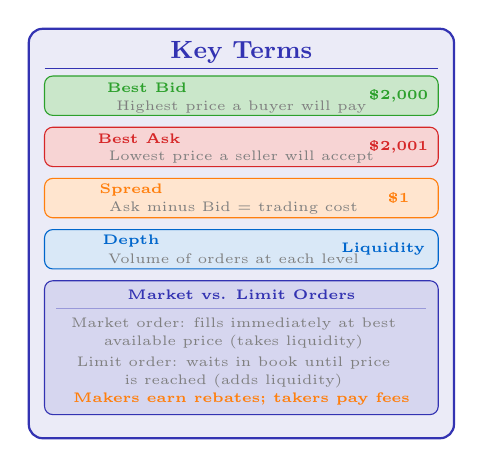
\begin{tikzpicture}
      % Key terms box
      \draw[fill=mlpurple!10, draw=mlpurple, rounded corners=5pt, thick]
           (0,0) rectangle (5.4,5.2);
      \node[font=\small\bfseries, mlpurple, align=center] at (2.7,4.9) {Key Terms};
      \draw[mlpurple, thin] (0.2,4.7) -- (5.2,4.7);

      % Best bid
      \draw[fill=mlgreen!25, draw=mlgreen, rounded corners=3pt] (0.2,4.1) rectangle (5.2,4.6);
      \node[font=\tiny\bfseries, mlgreen, align=left] at (1.5,4.45) {Best Bid};
      \node[font=\tiny, mlgray, align=left] at (2.7,4.2) {Highest price a buyer will pay};
      \node[font=\tiny\bfseries, mlgreen] at (4.7,4.35) {\$2{,}000};

      % Best ask
      \draw[fill=mlred!20, draw=mlred, rounded corners=3pt] (0.2,3.45) rectangle (5.2,3.95);
      \node[font=\tiny\bfseries, mlred, align=left] at (1.4,3.8) {Best Ask};
      \node[font=\tiny, mlgray, align=left] at (2.7,3.57) {Lowest price a seller will accept};
      \node[font=\tiny\bfseries, mlred] at (4.7,3.7) {\$2{,}001};

      % Spread
      \draw[fill=mlorange!20, draw=mlorange, rounded corners=3pt] (0.2,2.8) rectangle (5.2,3.3);
      \node[font=\tiny\bfseries, mlorange, align=left] at (1.3,3.15) {Spread};
      \node[font=\tiny, mlgray, align=left] at (2.6,2.92) {Ask minus Bid = trading cost};
      \node[font=\tiny\bfseries, mlorange] at (4.7,3.05) {\$1};

      % Depth
      \draw[fill=mlblue!15, draw=mlblue, rounded corners=3pt] (0.2,2.15) rectangle (5.2,2.65);
      \node[font=\tiny\bfseries, mlblue, align=left] at (1.3,2.5) {Depth};
      \node[font=\tiny, mlgray, align=left] at (2.6,2.28) {Volume of orders at each level};
      \node[font=\tiny\bfseries, mlblue] at (4.5,2.4) {Liquidity};

      % Market order note
      \draw[fill=mllavender4, draw=mlpurple, rounded corners=3pt] (0.2,0.3) rectangle (5.2,2.0);
      \node[font=\tiny\bfseries, mlpurple, align=center] at (2.7,1.82) {Market vs. Limit Orders};
      \draw[mlpurple!50, thin] (0.35,1.65) -- (5.05,1.65);
      \node[font=\tiny, mlgray, align=left] at (2.6,1.45) {Market order: fills immediately at best};
      \node[font=\tiny, mlgray, align=left] at (2.6,1.22) {available price (takes liquidity)};
      \node[font=\tiny, mlgray, align=left] at (2.6,0.95) {Limit order: waits in book until price};
      \node[font=\tiny, mlgray, align=left] at (2.6,0.72) {is reached (adds liquidity)};
      \node[font=\tiny\bfseries, mlorange, align=center] at (2.7,0.5) {Makers earn rebates; takers pay fees};
    \end{tikzpicture}
  \end{column}
\end{columns}

\bottomnote{The order book shows all resting buy and sell orders. The spread is the cost of an immediate trade; deep books mean high liquidity.}
\end{frame}

% ==================== FRAME 4: TRADING STRATEGIES FOR BEGINNERS ====================
\begin{frame}{Trading Strategies for Beginners}
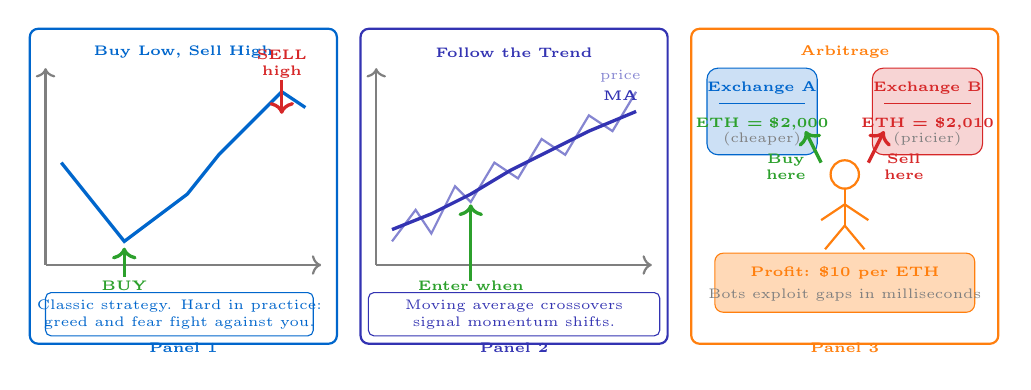
\begin{tikzpicture}
  % Panel borders
  \draw[thick, mlblue,   rounded corners=3pt] (0.1,0.2) rectangle (4.0,4.2);
  \draw[thick, mlpurple, rounded corners=3pt] (4.3,0.2) rectangle (8.2,4.2);
  \draw[thick, mlorange, rounded corners=3pt] (8.5,0.2) rectangle (12.4,4.2);

  % --- Panel 1: Buy Low, Sell High ---
  \node[font=\tiny\bfseries, mlblue] at (2.05,3.9) {Buy Low, Sell High};
  % Price wave
  \draw[->, mlgray, thick] (0.3,1.2) -- (3.8,1.2);
  \draw[->, mlgray, thick] (0.3,1.2) -- (0.3,3.7);
  % Price line dipping and recovering
  \draw[mlblue, very thick]
    (0.5,2.5) -- (0.9,2.0) -- (1.3,1.5) -- (1.7,1.8) -- (2.1,2.1) --
    (2.5,2.6) -- (2.9,3.0) -- (3.3,3.4) -- (3.6,3.2);
  % Buy arrow at dip
  \draw[->, very thick, mlgreen] (1.3,1.05) -- (1.3,1.42);
  \node[font=\tiny\bfseries, mlgreen, align=center] at (1.3,0.82) {BUY\\the dip};
  % Sell arrow at peak
  \draw[->, very thick, mlred] (3.3,3.55) -- (3.3,3.12);
  \node[font=\tiny\bfseries, mlred, align=center] at (3.3,3.75) {SELL\\high};
  % Speech bubble
  \draw[fill=white, draw=mlblue, rounded corners=2pt] (0.3,0.3) rectangle (3.7,0.85);
  \node[font=\tiny, mlblue, align=center] at (2.0,0.57) {Classic strategy. Hard in practice:\\greed and fear fight against you.};
  \node[font=\tiny\bfseries, mlblue] at (2.05,0.15) {Panel 1};

  % --- Panel 2: Follow the Trend ---
  \node[font=\tiny\bfseries, mlpurple] at (6.25,3.9) {Follow the Trend};
  % Axes
  \draw[->, mlgray, thick] (4.5,1.2) -- (8.0,1.2);
  \draw[->, mlgray, thick] (4.5,1.2) -- (4.5,3.7);
  % Price with uptrend noise
  \draw[mlpurple!60, thick]
    (4.7,1.5) -- (5.0,1.9) -- (5.2,1.6) -- (5.5,2.2) -- (5.7,2.0) --
    (6.0,2.5) -- (6.3,2.3) -- (6.6,2.8) -- (6.9,2.6) -- (7.2,3.1) --
    (7.5,2.9) -- (7.8,3.4);
  % Moving average line (smooth trend)
  \draw[mlpurple, very thick]
    (4.7,1.65) -- (5.2,1.85) -- (5.7,2.1) -- (6.2,2.4) -- (6.7,2.65) --
    (7.2,2.9) -- (7.8,3.15);
  % Label MA
  \node[font=\tiny\bfseries, mlpurple] at (7.6,3.35) {MA};
  \node[font=\tiny, mlpurple!60] at (7.6,3.6) {price};
  % Entry arrow
  \draw[->, very thick, mlgreen] (5.7,1.0) -- (5.7,1.97);
  \node[font=\tiny\bfseries, mlgreen, align=center] at (5.7,0.82) {Enter when\\price above MA};
  % Speech bubble
  \draw[fill=white, draw=mlpurple, rounded corners=2pt] (4.4,0.3) rectangle (8.1,0.85);
  \node[font=\tiny, mlpurple, align=center] at (6.25,0.57) {Moving average crossovers\\signal momentum shifts.};
  \node[font=\tiny\bfseries, mlpurple] at (6.25,0.15) {Panel 2};

  % --- Panel 3: Arbitrage ---
  \node[font=\tiny\bfseries, mlorange] at (10.45,3.9) {Arbitrage};
  % Exchange A box
  \draw[fill=mlblue!20, draw=mlblue, rounded corners=4pt] (8.7,2.6) rectangle (10.1,3.7);
  \node[font=\tiny\bfseries, mlblue, align=center] at (9.4,3.45) {Exchange A};
  \draw[mlblue, thin] (8.85,3.25) -- (9.95,3.25);
  \node[font=\tiny\bfseries, mlgreen, align=center] at (9.4,3.0) {ETH = \$2{,}000};
  \node[font=\tiny, mlgray, align=center] at (9.4,2.8) {(cheaper)};
  % Exchange B box
  \draw[fill=mlred!20, draw=mlred, rounded corners=4pt] (10.8,2.6) rectangle (12.2,3.7);
  \node[font=\tiny\bfseries, mlred, align=center] at (11.5,3.45) {Exchange B};
  \draw[mlred, thin] (10.95,3.25) -- (12.05,3.25);
  \node[font=\tiny\bfseries, mlred, align=center] at (11.5,3.0) {ETH = \$2{,}010};
  \node[font=\tiny, mlgray, align=center] at (11.5,2.8) {(pricier)};
  % Arbitrageur in middle
  \draw[mlorange, thick] (10.45,2.35) circle (0.18);
  \draw[mlorange, thick] (10.45,2.17) -- (10.45,1.70);
  \draw[mlorange, thick] (10.45,1.97) -- (10.15,1.77);
  \draw[mlorange, thick] (10.45,1.97) -- (10.75,1.77);
  \draw[mlorange, thick] (10.45,1.70) -- (10.20,1.40);
  \draw[mlorange, thick] (10.45,1.70) -- (10.70,1.40);
  % Arrows: buy on A, sell on B
  \draw[->, very thick, mlgreen]  (10.15,2.5) -- (9.95,2.9);
  \node[font=\tiny\bfseries, mlgreen, align=center] at (9.7,2.45) {Buy\\here};
  \draw[->, very thick, mlred]    (10.75,2.5) -- (10.95,2.9);
  \node[font=\tiny\bfseries, mlred, align=center] at (11.2,2.45) {Sell\\here};
  % Profit box
  \draw[fill=mlorange!30, draw=mlorange, rounded corners=3pt] (8.8,0.6) rectangle (12.1,1.35);
  \node[font=\tiny\bfseries, mlorange, align=center] at (10.45,1.1) {Profit: \$10 per ETH};
  \node[font=\tiny, mlgray, align=center] at (10.45,0.82) {Bots exploit gaps in milliseconds};
  \node[font=\tiny\bfseries, mlorange] at (10.45,0.15) {Panel 3};
\end{tikzpicture}

\bottomnote{Buy-low-sell-high requires timing skill; trend following uses indicators; arbitrage exploits price differences across venues.}
\end{frame}

% ==================== FRAME 5: WHAT IS RISK? ====================
\begin{frame}{What is Risk?}
\centering
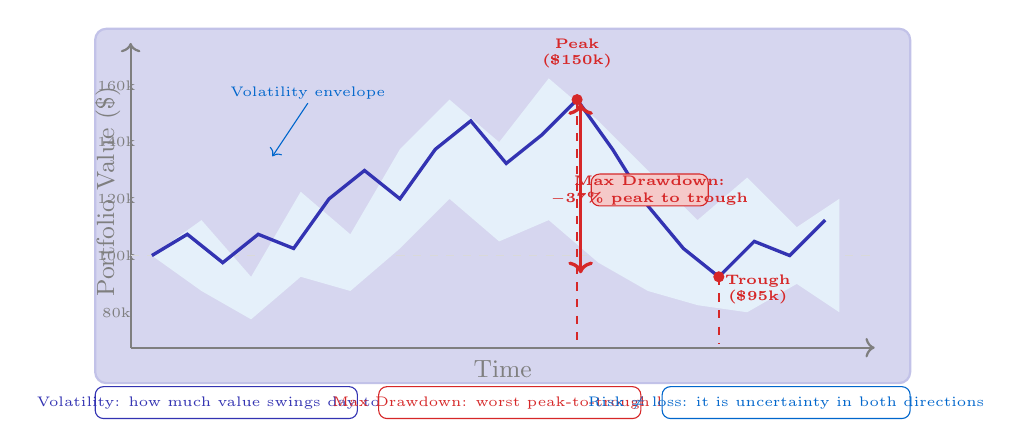
\begin{tikzpicture}[scale=0.90]
  % Chart background
  \draw[fill=mllavender4, draw=mlpurple!30, rounded corners=4pt, thick]
       (0,0.5) rectangle (11.5,5.5);

  % Axes
  \draw[->, mlgray, thick] (0.5,1.0) -- (11.0,1.0);
  \draw[->, mlgray, thick] (0.5,1.0) -- (0.5,5.3);
  \node[font=\small, mlgray, rotate=90] at (0.18,3.2) {Portfolio Value (\$)};
  \node[font=\small, mlgray] at (5.75,0.7) {Time};

  % Y-axis ticks
  \node[font=\tiny, mlgray] at (0.3,1.5) {80k};
  \node[font=\tiny, mlgray] at (0.3,2.3) {100k};
  \node[font=\tiny, mlgray] at (0.3,3.1) {120k};
  \node[font=\tiny, mlgray] at (0.3,3.9) {140k};
  \node[font=\tiny, mlgray] at (0.3,4.7) {160k};
  \draw[mlgray!30, dashed, thin] (0.5,2.3) -- (11.0,2.3);

  % Volatility envelope (shaded band)
  \fill[mlblue!10]
    (0.8,2.3) -- (1.5,2.8) -- (2.2,2.0) -- (2.9,3.2) -- (3.6,2.6) --
    (4.3,3.8) -- (5.0,4.5) -- (5.7,3.9) -- (6.4,4.8) -- (7.1,4.2) --
    (7.8,3.5) -- (8.5,2.8) -- (9.2,3.4) -- (9.9,2.7) -- (10.5,3.1) --
    (10.5,1.5) -- (9.9,1.9) -- (9.2,1.5) -- (8.5,1.6) -- (7.8,1.8) --
    (7.1,2.2) -- (6.4,2.8) -- (5.7,2.5) -- (5.0,3.1) -- (4.3,2.4) --
    (3.6,1.8) -- (2.9,2.0) -- (2.2,1.4) -- (1.5,1.8) -- (0.8,2.3) -- cycle;

  % Main portfolio value line
  \draw[mlpurple, very thick]
    (0.8,2.3) -- (1.3,2.6) -- (1.8,2.2) -- (2.3,2.6) -- (2.8,2.4) --
    (3.3,3.1) -- (3.8,3.5) -- (4.3,3.1) -- (4.8,3.8) -- (5.3,4.2) --
    (5.8,3.6) -- (6.3,4.0) -- (6.8,4.5) -- (7.3,3.8) -- (7.8,3.0) --
    (8.3,2.4) -- (8.8,2.0) -- (9.3,2.5) -- (9.8,2.3) -- (10.3,2.8);

  % Peak marker
  \draw[mlred, dashed, thick] (6.8,4.5) -- (6.8,1.05);
  \draw[fill=mlred, draw=mlred] (6.8,4.5) circle (0.07);
  \node[font=\tiny\bfseries, mlred, align=center] at (6.8,5.15) {Peak\\(\$150k)};

  % Trough marker
  \draw[mlred, dashed, thick] (8.8,2.0) -- (8.8,1.05);
  \draw[fill=mlred, draw=mlred] (8.8,2.0) circle (0.07);
  \node[font=\tiny\bfseries, mlred, align=center] at (9.35,1.82) {Trough\\(\$95k)};

  % Max drawdown brace / arrow
  \draw[<->, very thick, mlred] (6.85,2.05) -- (6.85,4.45);
  \draw[fill=mlred!25, draw=mlred, rounded corners=3pt] (7.0,3.0) rectangle (8.65,3.45);
  \node[font=\tiny\bfseries, mlred, align=center] at (7.82,3.22) {Max Drawdown:\\$-$37\% peak to trough};

  % Volatility envelope label
  \node[font=\tiny, mlblue, align=center] at (3.0,4.6) {Volatility envelope};
  \draw[->, thin, mlblue] (3.0,4.45) -- (2.5,3.7);

  % Risk explanation boxes
  \draw[fill=white, draw=mlpurple, rounded corners=3pt] (0.0,0.0) rectangle (3.7,0.45);
  \node[font=\tiny, mlpurple, align=center] at (1.85,0.22) {Volatility: how much value swings day to day};

  \draw[fill=white, draw=mlred, rounded corners=3pt] (4.0,0.0) rectangle (7.7,0.45);
  \node[font=\tiny, mlred, align=center] at (5.85,0.22) {Max Drawdown: worst peak-to-trough loss};

  \draw[fill=white, draw=mlblue, rounded corners=3pt] (8.0,0.0) rectangle (11.5,0.45);
  \node[font=\tiny, mlblue, align=center] at (9.75,0.22) {Risk $\neq$ loss: it is uncertainty in both directions};
\end{tikzpicture}

\bottomnote{Risk in crypto is measured as volatility (price swings) and max drawdown (worst loss from peak). High return often means high risk.}
\end{frame}

% ==================== FRAME 6: THE SHARPE RATIO EXPLAINED ====================
\begin{frame}{The Sharpe Ratio Explained}
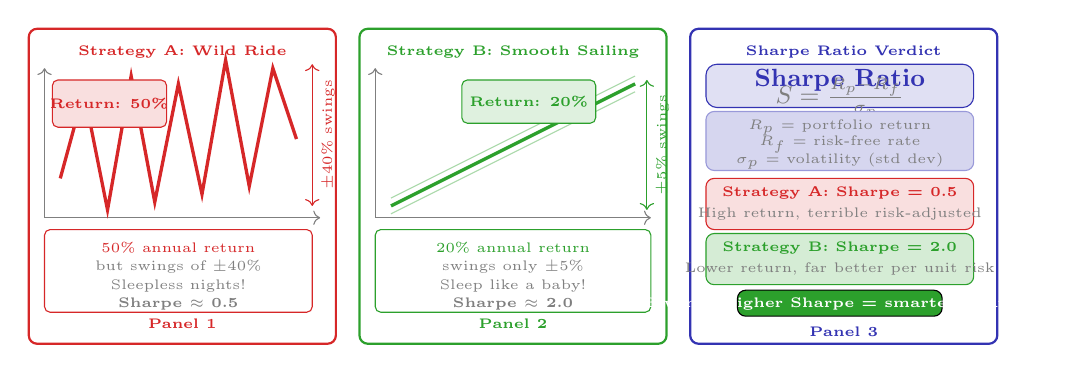
\begin{tikzpicture}
  % Panel borders
  \draw[thick, mlred,    rounded corners=3pt] (0.1,0.2) rectangle (4.0,4.2);
  \draw[thick, mlgreen,  rounded corners=3pt] (4.3,0.2) rectangle (8.2,4.2);
  \draw[thick, mlpurple, rounded corners=3pt] (8.5,0.2) rectangle (12.4,4.2);

  % --- Panel 1: Strategy A: high return, wild swings ---
  \node[font=\tiny\bfseries, mlred] at (2.05,3.9) {Strategy A: Wild Ride};
  % Chart axes
  \draw[->, mlgray, thin] (0.3,1.8) -- (3.8,1.8);
  \draw[->, mlgray, thin] (0.3,1.8) -- (0.3,3.7);
  % Volatile line
  \draw[mlred, very thick]
    (0.5,2.3) -- (0.8,3.4) -- (1.1,1.9) -- (1.4,3.6) -- (1.7,2.0) --
    (2.0,3.5) -- (2.3,2.1) -- (2.6,3.8) -- (2.9,2.2) -- (3.2,3.7) --
    (3.5,2.8);
  % Return label
  \draw[fill=mlred!15, draw=mlred, rounded corners=2pt] (0.4,2.95) rectangle (1.85,3.55);
  \node[font=\tiny\bfseries, mlred, align=center] at (1.12,3.25) {Return: 50\%};
  % Swing annotation
  \draw[<->, mlred, thin] (3.7,1.95) -- (3.7,3.75);
  \node[font=\tiny, mlred, rotate=90] at (3.9,2.85) {$\pm40\%$ swings};
  % Speech bubble
  \draw[fill=white, draw=mlred, rounded corners=2pt] (0.3,0.6) rectangle (3.7,1.65);
  \node[font=\tiny, mlred, align=center] at (2.0,1.42) {50\% annual return};
  \node[font=\tiny, mlgray, align=center] at (2.0,1.18) {but swings of $\pm40\%$};
  \node[font=\tiny, mlgray, align=center] at (2.0,0.93) {Sleepless nights!};
  \node[font=\tiny\bfseries, mlgray, align=center] at (2.0,0.70) {Sharpe $\approx$ 0.5};
  \node[font=\tiny\bfseries, mlred] at (2.05,0.45) {Panel 1};

  % --- Panel 2: Strategy B: modest return, smooth ---
  \node[font=\tiny\bfseries, mlgreen] at (6.25,3.9) {Strategy B: Smooth Sailing};
  % Chart axes
  \draw[->, mlgray, thin] (4.5,1.8) -- (8.0,1.8);
  \draw[->, mlgray, thin] (4.5,1.8) -- (4.5,3.7);
  % Smooth upward line
  \draw[mlgreen, very thick]
    (4.7,1.95) -- (5.1,2.15) -- (5.5,2.35) -- (5.9,2.55) -- (6.3,2.75) --
    (6.7,2.95) -- (7.1,3.15) -- (7.5,3.35) -- (7.8,3.5);
  % Minor band
  \draw[mlgreen!40, thin]
    (4.7,2.05) -- (5.1,2.25) -- (5.5,2.45) -- (5.9,2.65) -- (6.3,2.85) --
    (6.7,3.05) -- (7.1,3.25) -- (7.5,3.45) -- (7.8,3.6);
  \draw[mlgreen!40, thin]
    (4.7,1.85) -- (5.1,2.05) -- (5.5,2.25) -- (5.9,2.45) -- (6.3,2.65) --
    (6.7,2.85) -- (7.1,3.05) -- (7.5,3.25) -- (7.8,3.4);
  % Return label
  \draw[fill=mlgreen!15, draw=mlgreen, rounded corners=2pt] (5.6,3.0) rectangle (7.3,3.55);
  \node[font=\tiny\bfseries, mlgreen, align=center] at (6.45,3.27) {Return: 20\%};
  % Swing annotation
  \draw[<->, mlgreen, thin] (7.95,1.9) -- (7.95,3.55);
  \node[font=\tiny, mlgreen, rotate=90] at (8.15,2.72) {$\pm5\%$ swings};
  % Speech bubble
  \draw[fill=white, draw=mlgreen, rounded corners=2pt] (4.5,0.6) rectangle (8.0,1.65);
  \node[font=\tiny, mlgreen, align=center] at (6.25,1.42) {20\% annual return};
  \node[font=\tiny, mlgray, align=center] at (6.25,1.18) {swings only $\pm5\%$};
  \node[font=\tiny, mlgray, align=center] at (6.25,0.93) {Sleep like a baby!};
  \node[font=\tiny\bfseries, mlgray, align=center] at (6.25,0.70) {Sharpe $\approx$ 2.0};
  \node[font=\tiny\bfseries, mlgreen] at (6.25,0.45) {Panel 2};

  % --- Panel 3: Sharpe says B wins ---
  \node[font=\tiny\bfseries, mlpurple] at (10.45,3.9) {Sharpe Ratio Verdict};
  % Formula box
  \draw[fill=mlpurple!15, draw=mlpurple, rounded corners=4pt] (8.7,3.2) rectangle (12.1,3.75);
  \node[font=\small\bfseries, mlpurple, align=center] at (10.4,3.55) {Sharpe Ratio};
  \node[font=\small, mlgray, align=center] at (10.4,3.32) {$S = \frac{R_p - R_f}{\sigma_p}$};

  % Explanation
  \draw[fill=mllavender4, draw=mlpurple!50, rounded corners=3pt] (8.7,2.4) rectangle (12.1,3.15);
  \node[font=\tiny, mlgray, align=center] at (10.4,2.95) {$R_p$ = portfolio return};
  \node[font=\tiny, mlgray, align=center] at (10.4,2.73) {$R_f$ = risk-free rate};
  \node[font=\tiny, mlgray, align=center] at (10.4,2.52) {$\sigma_p$ = volatility (std dev)};

  % Comparison result
  \draw[fill=mlred!15, draw=mlred, rounded corners=3pt] (8.7,1.65) rectangle (12.1,2.3);
  \node[font=\tiny\bfseries, mlred, align=center] at (10.4,2.12) {Strategy A: Sharpe = 0.5};
  \node[font=\tiny, mlgray, align=center] at (10.4,1.85) {High return, terrible risk-adjusted};

  \draw[fill=mlgreen!20, draw=mlgreen, rounded corners=3pt] (8.7,0.95) rectangle (12.1,1.6);
  \node[font=\tiny\bfseries, mlgreen, align=center] at (10.4,1.42) {Strategy B: Sharpe = 2.0};
  \node[font=\tiny, mlgray, align=center] at (10.4,1.15) {Lower return, far better per unit risk};

  % Winner badge
  \draw[fill=mlgreen, rounded corners=3pt] (9.1,0.55) rectangle (11.7,0.88);
  \node[font=\tiny\bfseries, white, align=center] at (10.4,0.71) {B wins! Higher Sharpe = smarter strategy};
  \node[font=\tiny\bfseries, mlpurple] at (10.45,0.35) {Panel 3};
\end{tikzpicture}

\bottomnote{Sharpe Ratio = (Return $-$ Risk-Free Rate) / Volatility. A higher Sharpe means more return per unit of risk. Target Sharpe $>$ 1.}
\end{frame}

% ==================== FRAME 7: CEX VS DEX ====================
\begin{frame}{CEX vs.\ DEX}
\centering
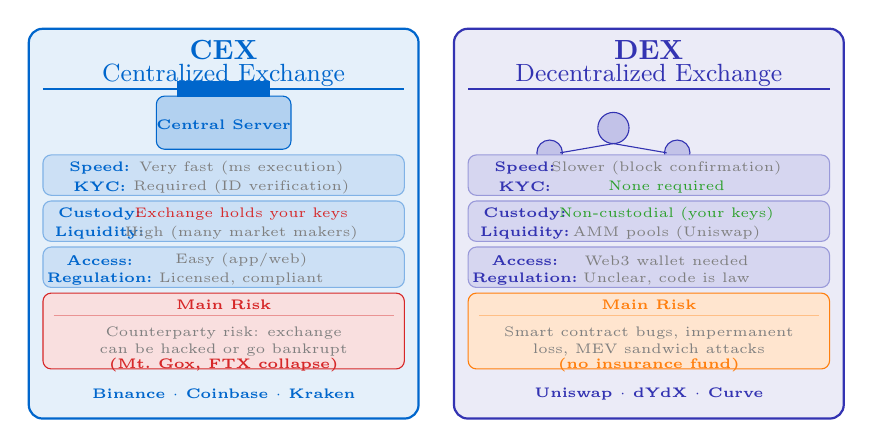
\begin{tikzpicture}[scale=0.90]
  % Background for CEX
  \draw[fill=mlblue!10, draw=mlblue, rounded corners=5pt, thick]
       (0,0.0) rectangle (5.5,5.5);
  \node[font=\normalsize\bfseries, mlblue, align=center] at (2.75,5.2)
       {CEX};
  \node[font=\small, mlblue, align=center] at (2.75,4.85)
       {Centralized Exchange};
  \draw[mlblue, thin] (0.2,4.65) -- (5.3,4.65);

  % CEX icon: building / server
  \draw[fill=mlblue!30, draw=mlblue, rounded corners=3pt] (1.8,3.8) rectangle (3.7,4.55);
  \draw[fill=mlblue, draw=mlblue] (2.1,4.55) rectangle (3.4,4.75);
  \node[font=\tiny\bfseries, mlblue, align=center] at (2.75,4.15) {Central Server};

  % CEX properties
  \draw[fill=mlblue!20, draw=mlblue!50, rounded corners=3pt] (0.2,3.15) rectangle (5.3,3.72);
  \node[font=\tiny\bfseries, mlblue, align=left] at (1.0,3.53) {Speed:};
  \node[font=\tiny, mlgray, align=left] at (3.0,3.53) {Very fast (ms execution)};
  \node[font=\tiny\bfseries, mlblue, align=left] at (1.0,3.27) {KYC:};
  \node[font=\tiny, mlgray, align=left] at (3.0,3.27) {Required (ID verification)};

  \draw[fill=mlblue!20, draw=mlblue!50, rounded corners=3pt] (0.2,2.5) rectangle (5.3,3.07);
  \node[font=\tiny\bfseries, mlblue, align=left] at (1.0,2.88) {Custody:};
  \node[font=\tiny, mlred, align=left] at (3.0,2.88) {Exchange holds your keys};
  \node[font=\tiny\bfseries, mlblue, align=left] at (1.0,2.62) {Liquidity:};
  \node[font=\tiny, mlgray, align=left] at (3.0,2.62) {High (many market makers)};

  \draw[fill=mlblue!20, draw=mlblue!50, rounded corners=3pt] (0.2,1.85) rectangle (5.3,2.42);
  \node[font=\tiny\bfseries, mlblue, align=left] at (1.0,2.23) {Access:};
  \node[font=\tiny, mlgray, align=left] at (3.0,2.23) {Easy (app/web)};
  \node[font=\tiny\bfseries, mlblue, align=left] at (1.0,1.97) {Regulation:};
  \node[font=\tiny, mlgray, align=left] at (3.0,1.97) {Licensed, compliant};

  % Risk box
  \draw[fill=mlred!15, draw=mlred, rounded corners=3pt] (0.2,0.7) rectangle (5.3,1.77);
  \node[font=\tiny\bfseries, mlred, align=center] at (2.75,1.6) {Main Risk};
  \draw[mlred!50, thin] (0.35,1.45) -- (5.15,1.45);
  \node[font=\tiny, mlgray, align=center] at (2.75,1.2) {Counterparty risk: exchange};
  \node[font=\tiny, mlgray, align=center] at (2.75,0.97) {can be hacked or go bankrupt};
  \node[font=\tiny\bfseries, mlred, align=center] at (2.75,0.75) {(Mt.\ Gox, FTX collapse)};

  % Examples
  \node[font=\tiny\bfseries, mlblue, align=center] at (2.75,0.35)
       {Binance $\cdot$ Coinbase $\cdot$ Kraken};

  % Background for DEX
  \draw[fill=mlpurple!10, draw=mlpurple, rounded corners=5pt, thick]
       (6.0,0.0) rectangle (11.5,5.5);
  \node[font=\normalsize\bfseries, mlpurple, align=center] at (8.75,5.2)
       {DEX};
  \node[font=\small, mlpurple, align=center] at (8.75,4.85)
       {Decentralized Exchange};
  \draw[mlpurple, thin] (6.2,4.65) -- (11.3,4.65);

  % DEX icon: nodes network
  \draw[fill=mlpurple!30, draw=mlpurple] (8.25,4.1) circle (0.22);
  \draw[fill=mlpurple!30, draw=mlpurple] (7.35,3.75) circle (0.18);
  \draw[fill=mlpurple!30, draw=mlpurple] (9.15,3.75) circle (0.18);
  \draw[fill=mlpurple!30, draw=mlpurple] (7.6,3.4) circle (0.15);
  \draw[fill=mlpurple!30, draw=mlpurple] (8.9,3.4) circle (0.15);
  \draw[mlpurple, thin] (8.25,3.88) -- (7.5,3.75);
  \draw[mlpurple, thin] (8.25,3.88) -- (9.0,3.75);
  \draw[mlpurple, thin] (7.5,3.57) -- (7.65,3.42);
  \draw[mlpurple, thin] (9.0,3.57) -- (8.88,3.42);
  \draw[mlpurple, thin] (7.65,3.42) -- (8.88,3.42);

  % DEX properties
  \draw[fill=mlpurple!20, draw=mlpurple!50, rounded corners=3pt] (6.2,3.15) rectangle (11.3,3.72);
  \node[font=\tiny\bfseries, mlpurple, align=left] at (7.0,3.53) {Speed:};
  \node[font=\tiny, mlgray, align=left] at (9.0,3.53) {Slower (block confirmation)};
  \node[font=\tiny\bfseries, mlpurple, align=left] at (7.0,3.27) {KYC:};
  \node[font=\tiny, mlgreen, align=left] at (9.0,3.27) {None required};

  \draw[fill=mlpurple!20, draw=mlpurple!50, rounded corners=3pt] (6.2,2.5) rectangle (11.3,3.07);
  \node[font=\tiny\bfseries, mlpurple, align=left] at (7.0,2.88) {Custody:};
  \node[font=\tiny, mlgreen, align=left] at (9.0,2.88) {Non-custodial (your keys)};
  \node[font=\tiny\bfseries, mlpurple, align=left] at (7.0,2.62) {Liquidity:};
  \node[font=\tiny, mlgray, align=left] at (9.0,2.62) {AMM pools (Uniswap)};

  \draw[fill=mlpurple!20, draw=mlpurple!50, rounded corners=3pt] (6.2,1.85) rectangle (11.3,2.42);
  \node[font=\tiny\bfseries, mlpurple, align=left] at (7.0,2.23) {Access:};
  \node[font=\tiny, mlgray, align=left] at (9.0,2.23) {Web3 wallet needed};
  \node[font=\tiny\bfseries, mlpurple, align=left] at (7.0,1.97) {Regulation:};
  \node[font=\tiny, mlgray, align=left] at (9.0,1.97) {Unclear, code is law};

  % Risk box
  \draw[fill=mlorange!20, draw=mlorange, rounded corners=3pt] (6.2,0.7) rectangle (11.3,1.77);
  \node[font=\tiny\bfseries, mlorange, align=center] at (8.75,1.6) {Main Risk};
  \draw[mlorange!50, thin] (6.35,1.45) -- (11.15,1.45);
  \node[font=\tiny, mlgray, align=center] at (8.75,1.2) {Smart contract bugs, impermanent};
  \node[font=\tiny, mlgray, align=center] at (8.75,0.97) {loss, MEV sandwich attacks};
  \node[font=\tiny\bfseries, mlorange, align=center] at (8.75,0.75) {(no insurance fund)};

  % Examples
  \node[font=\tiny\bfseries, mlpurple, align=center] at (8.75,0.35)
       {Uniswap $\cdot$ dYdX $\cdot$ Curve};
\end{tikzpicture}

\bottomnote{CEX offers speed and ease but requires trust in the operator. DEX is trustless and non-custodial but slower and technically demanding.}
\end{frame}

% ==================== FRAME 8: MARKET MANIPULATION ====================
\begin{frame}{Market Manipulation}
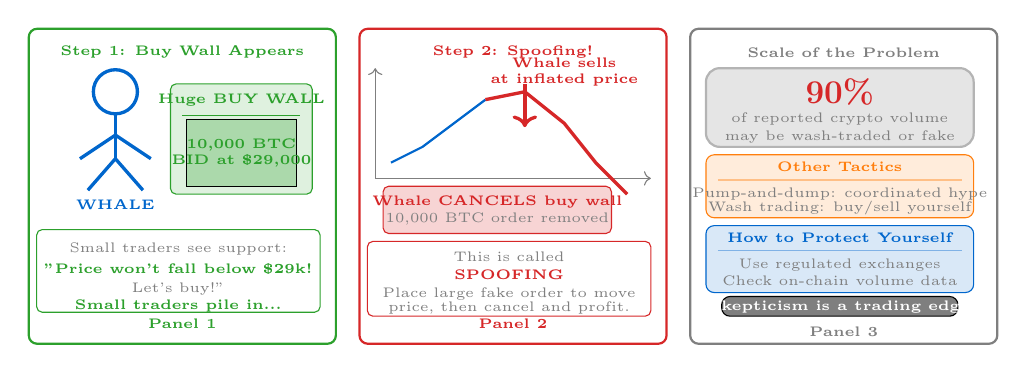
\begin{tikzpicture}
  % Panel borders
  \draw[thick, mlgreen,  rounded corners=3pt] (0.1,0.2) rectangle (4.0,4.2);
  \draw[thick, mlred,    rounded corners=3pt] (4.3,0.2) rectangle (8.2,4.2);
  \draw[thick, mlgray,   rounded corners=3pt] (8.5,0.2) rectangle (12.4,4.2);

  % --- Panel 1: Whale places buy wall ---
  \node[font=\tiny\bfseries, mlgreen] at (2.05,3.9) {Step 1: Buy Wall Appears};
  % Whale figure (large)
  \draw[mlblue, very thick] (1.2,3.4) circle (0.28);
  \draw[mlblue, very thick] (1.2,3.12) -- (1.2,2.55);
  \draw[mlblue, very thick] (1.2,2.85) -- (0.75,2.55);
  \draw[mlblue, very thick] (1.2,2.85) -- (1.65,2.55);
  \draw[mlblue, very thick] (1.2,2.55) -- (0.85,2.15);
  \draw[mlblue, very thick] (1.2,2.55) -- (1.55,2.15);
  \node[font=\tiny\bfseries, mlblue] at (1.2,1.97) {WHALE};
  % Order book with big green wall
  \draw[fill=mlgreen!15, draw=mlgreen, rounded corners=2pt] (1.9,2.1) rectangle (3.7,3.5);
  \node[font=\tiny\bfseries, mlgreen, align=center] at (2.8,3.3) {Huge BUY WALL};
  \draw[mlgreen, thin] (2.05,3.1) -- (3.55,3.1);
  \draw[fill=mlgreen!40] (2.1,2.2) rectangle (3.5,3.05);
  \node[font=\tiny\bfseries, mlgreen, align=center] at (2.8,2.62) {10{,}000 BTC\\BID at \$29{,}000};
  % Small traders look at wall
  \draw[fill=white, draw=mlgreen, rounded corners=2pt] (0.2,0.6) rectangle (3.8,1.65);
  \node[font=\tiny, mlgray, align=center] at (2.0,1.4) {Small traders see support:};
  \node[font=\tiny\bfseries, mlgreen, align=center] at (2.0,1.15) {"Price won't fall below \$29k!};
  \node[font=\tiny, mlgray, align=center] at (2.0,0.9) {Let's buy!''};
  \node[font=\tiny\bfseries, mlgreen, align=center] at (2.0,0.68) {Small traders pile in...};
  \node[font=\tiny\bfseries, mlgreen] at (2.05,0.45) {Panel 1};

  % --- Panel 2: Whale cancels and sells - spoofing ---
  \node[font=\tiny\bfseries, mlred] at (6.25,3.9) {Step 2: Spoofing!};
  % Price chart - rises then crashes
  \draw[->, mlgray, thin] (4.5,2.3) -- (8.0,2.3);
  \draw[->, mlgray, thin] (4.5,2.3) -- (4.5,3.7);
  \draw[mlblue, thick] (4.7,2.5) -- (5.1,2.7) -- (5.5,3.0) -- (5.9,3.3);
  \draw[mlred, very thick] (5.9,3.3) -- (6.4,3.4) -- (6.9,3.0) -- (7.3,2.5) -- (7.7,2.1);
  % Cancel order cross
  \draw[fill=mlred!20, draw=mlred, rounded corners=2pt] (4.6,1.6) rectangle (7.5,2.2);
  \node[font=\tiny\bfseries, mlred, align=center] at (6.05,2.0) {Whale CANCELS buy wall};
  \node[font=\tiny, mlgray, align=center] at (6.05,1.78) {10{,}000 BTC order removed};
  % Whale sells at top arrow
  \draw[->, very thick, mlred] (6.4,3.5) -- (6.4,2.95);
  \node[font=\tiny\bfseries, mlred, align=center] at (6.9,3.65) {Whale sells\\at inflated price};
  % Explanation
  \draw[fill=white, draw=mlred, rounded corners=2pt] (4.4,0.55) rectangle (8.0,1.5);
  \node[font=\tiny, mlgray, align=center] at (6.2,1.3) {This is called};
  \node[font=\tiny\bfseries, mlred, align=center] at (6.2,1.07) {SPOOFING};
  \node[font=\tiny, mlgray, align=center] at (6.2,0.83) {Place large fake order to move};
  \node[font=\tiny, mlgray, align=center] at (6.2,0.65) {price, then cancel and profit.};
  \node[font=\tiny\bfseries, mlred] at (6.25,0.45) {Panel 2};

  % --- Panel 3: Fake volume stat ---
  \node[font=\tiny\bfseries, mlgray] at (10.45,3.9) {Scale of the Problem};
  % Large stat display
  \draw[fill=mlgray!20, draw=midgray, rounded corners=5pt, thick]
       (8.7,2.7) rectangle (12.1,3.7);
  \node[font=\large\bfseries, mlred, align=center] at (10.4,3.4) {90\%};
  \node[font=\tiny, mlgray, align=center] at (10.4,3.05) {of reported crypto volume};
  \node[font=\tiny, mlgray, align=center] at (10.4,2.82) {may be wash-traded or fake};
  % Other manipulation types
  \draw[fill=mlorange!15, draw=mlorange, rounded corners=3pt] (8.7,1.8) rectangle (12.1,2.6);
  \node[font=\tiny\bfseries, mlorange, align=center] at (10.4,2.45) {Other Tactics};
  \draw[mlorange!50, thin] (8.85,2.28) -- (11.95,2.28);
  \node[font=\tiny, mlgray, align=center] at (10.4,2.1) {Pump-and-dump: coordinated hype};
  \node[font=\tiny, mlgray, align=center] at (10.4,1.92) {Wash trading: buy/sell yourself};
  % Protection advice
  \draw[fill=mlblue!15, draw=mlblue, rounded corners=3pt] (8.7,0.85) rectangle (12.1,1.7);
  \node[font=\tiny\bfseries, mlblue, align=center] at (10.4,1.55) {How to Protect Yourself};
  \draw[mlblue!50, thin] (8.85,1.38) -- (11.95,1.38);
  \node[font=\tiny, mlgray, align=center] at (10.4,1.2) {Use regulated exchanges};
  \node[font=\tiny, mlgray, align=center] at (10.4,1.0) {Check on-chain volume data};
  \draw[fill=mlgray, rounded corners=3pt] (8.9,0.55) rectangle (11.9,0.8);
  \node[font=\tiny\bfseries, white, align=center] at (10.4,0.67) {Skepticism is a trading edge};
  \node[font=\tiny\bfseries, mlgray] at (10.45,0.35) {Panel 3};
\end{tikzpicture}

\bottomnote{Market manipulation is rampant in crypto. Spoofing, wash trading, and pump-and-dump schemes distort prices and harm retail investors.}
\end{frame}

% ==================== FRAME 9: REGULATION IS COMING ====================
\begin{frame}{Regulation is Coming}
\centering
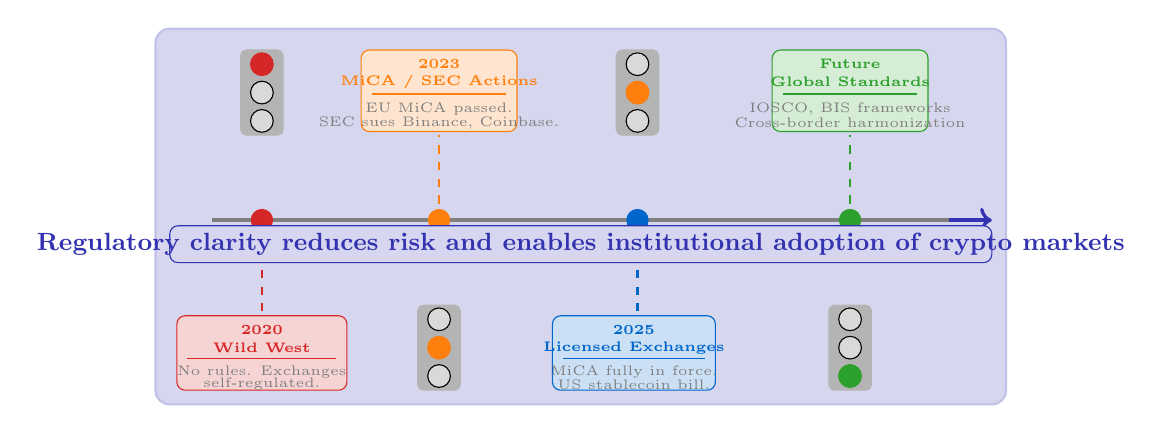
\begin{tikzpicture}[scale=0.90]
  % Background
  \draw[fill=mllavender4, draw=mlpurple!30, rounded corners=5pt, thick]
       (0,0.3) rectangle (12.0,5.6);

  % Timeline axis
  \draw[very thick, mlgray] (0.8,2.9) -- (11.2,2.9);
  \draw[->, very thick, mlpurple] (11.2,2.9) -- (11.8,2.9);
  \node[font=\small\bfseries, mlpurple] at (11.7,3.2) {};

  % --- Node 1: 2020 Wild West ---
  \draw[fill=mlred, draw=mlred] (1.5,2.9) circle (0.15);
  \draw[mlred, dashed, thick] (1.5,2.9) -- (1.5,1.6);
  \draw[fill=mlred!20, draw=mlred, rounded corners=3pt] (0.3,0.5) rectangle (2.7,1.55);
  \node[font=\tiny\bfseries, mlred, align=center] at (1.5,1.35) {2020};
  \node[font=\tiny\bfseries, mlred, align=center] at (1.5,1.1) {Wild West};
  \draw[mlred, thin] (0.45,0.95) -- (2.55,0.95);
  \node[font=\tiny, mlgray, align=center] at (1.5,0.75) {No rules. Exchanges};
  \node[font=\tiny, mlgray, align=center] at (1.5,0.58) {self-regulated.};
  % Traffic light: red
  \draw[fill=midgray, draw=midgray, rounded corners=2pt] (1.2,4.1) rectangle (1.8,5.3);
  \draw[fill=mlred, draw=mlred] (1.5,5.1) circle (0.16);
  \draw[fill=midgray!50] (1.5,4.7) circle (0.16);
  \draw[fill=midgray!50] (1.5,4.3) circle (0.16);

  % --- Node 2: 2023 MiCA / SEC ---
  \draw[fill=mlorange, draw=mlorange] (4.0,2.9) circle (0.15);
  \draw[mlorange, dashed, thick] (4.0,2.9) -- (4.0,4.1);
  \draw[fill=mlorange!20, draw=mlorange, rounded corners=3pt] (2.9,4.15) rectangle (5.1,5.3);
  \node[font=\tiny\bfseries, mlorange, align=center] at (4.0,5.1) {2023};
  \node[font=\tiny\bfseries, mlorange, align=center] at (4.0,4.85) {MiCA / SEC Actions};
  \draw[mlorange, thin] (3.05,4.68) -- (4.95,4.68);
  \node[font=\tiny, mlgray, align=center] at (4.0,4.47) {EU MiCA passed.};
  \node[font=\tiny, mlgray, align=center] at (4.0,4.27) {SEC sues Binance, Coinbase.};
  % Traffic light: orange
  \draw[fill=midgray, draw=midgray, rounded corners=2pt] (3.7,0.5) rectangle (4.3,1.7);
  \draw[fill=midgray!50] (4.0,1.5) circle (0.16);
  \draw[fill=mlorange, draw=mlorange] (4.0,1.1) circle (0.16);
  \draw[fill=midgray!50] (4.0,0.7) circle (0.16);

  % --- Node 3: 2025 Licensed exchanges ---
  \draw[fill=mlblue, draw=mlblue] (6.8,2.9) circle (0.15);
  \draw[mlblue, dashed, thick] (6.8,2.9) -- (6.8,1.6);
  \draw[fill=mlblue!20, draw=mlblue, rounded corners=3pt] (5.6,0.5) rectangle (7.9,1.55);
  \node[font=\tiny\bfseries, mlblue, align=center] at (6.75,1.35) {2025};
  \node[font=\tiny\bfseries, mlblue, align=center] at (6.75,1.1) {Licensed Exchanges};
  \draw[mlblue, thin] (5.75,0.95) -- (7.75,0.95);
  \node[font=\tiny, mlgray, align=center] at (6.75,0.75) {MiCA fully in force.};
  \node[font=\tiny, mlgray, align=center] at (6.75,0.58) {US stablecoin bill.};
  % Traffic light: amber/transitioning
  \draw[fill=midgray, draw=midgray, rounded corners=2pt] (6.5,4.1) rectangle (7.1,5.3);
  \draw[fill=midgray!50] (6.8,5.1) circle (0.16);
  \draw[fill=mlorange, draw=mlorange] (6.8,4.7) circle (0.16);
  \draw[fill=midgray!50] (6.8,4.3) circle (0.16);

  % --- Node 4: Future Global standards ---
  \draw[fill=mlgreen, draw=mlgreen] (9.8,2.9) circle (0.15);
  \draw[mlgreen, dashed, thick] (9.8,2.9) -- (9.8,4.1);
  \draw[fill=mlgreen!20, draw=mlgreen, rounded corners=3pt] (8.7,4.15) rectangle (10.9,5.3);
  \node[font=\tiny\bfseries, mlgreen, align=center] at (9.8,5.1) {Future};
  \node[font=\tiny\bfseries, mlgreen, align=center] at (9.8,4.85) {Global Standards};
  \draw[mlgreen, thin] (8.85,4.68) -- (10.75,4.68);
  \node[font=\tiny, mlgray, align=center] at (9.8,4.47) {IOSCO, BIS frameworks};
  \node[font=\tiny, mlgray, align=center] at (9.8,4.27) {Cross-border harmonization};
  % Traffic light: green
  \draw[fill=midgray, draw=midgray, rounded corners=2pt] (9.5,0.5) rectangle (10.1,1.7);
  \draw[fill=midgray!50] (9.8,1.5) circle (0.16);
  \draw[fill=midgray!50] (9.8,1.1) circle (0.16);
  \draw[fill=mlgreen, draw=mlgreen] (9.8,0.7) circle (0.16);

  % Summary bar
  \draw[fill=mlpurple!20, draw=mlpurple, rounded corners=3pt] (0.2,2.3) rectangle (11.8,2.82);
  \node[font=\small\bfseries, mlpurple, align=center] at (6.0,2.56)
       {Regulatory clarity reduces risk and enables institutional adoption of crypto markets};
\end{tikzpicture}

\bottomnote{Crypto is transitioning from a largely unregulated space to a licensed industry. MiCA (EU) and SEC enforcement mark the turning point.}
\end{frame}

% ==================== FRAME 10: KEY TAKEAWAYS ====================
\begin{frame}{Key Takeaways}
\centering
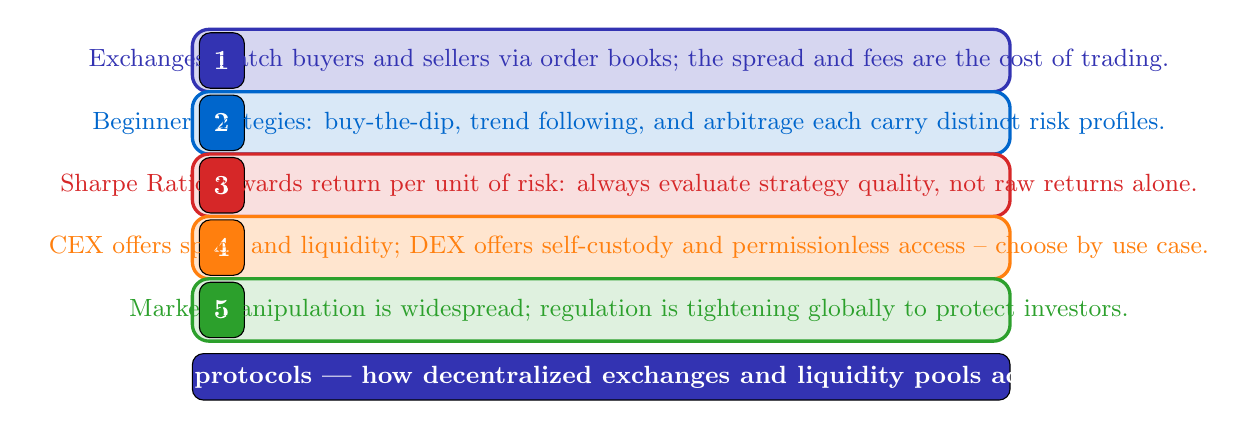
\begin{tikzpicture}[scale=0.88]
  % Box 1
  \draw[fill=mlpurple!20, draw=mlpurple, very thick, rounded corners=6pt]
       (0,4.0) rectangle (11.8,4.9);
  \draw[fill=mlpurple, rounded corners=4pt] (0.1,4.05) rectangle (0.75,4.85);
  \node[font=\normalsize\bfseries, white] at (0.42,4.45) {1};
  \node[font=\small, mlpurple, align=left] at (6.3,4.45)
       {Exchanges match buyers and sellers via order books; the spread and fees are the cost of trading.};

  % Box 2
  \draw[fill=mlblue!15, draw=mlblue, very thick, rounded corners=6pt]
       (0,3.1) rectangle (11.8,4.0);
  \draw[fill=mlblue, rounded corners=4pt] (0.1,3.15) rectangle (0.75,3.95);
  \node[font=\normalsize\bfseries, white] at (0.42,3.55) {2};
  \node[font=\small, mlblue, align=left] at (6.3,3.55)
       {Beginner strategies: buy-the-dip, trend following, and arbitrage each carry distinct risk profiles.};

  % Box 3
  \draw[fill=mlred!15, draw=mlred, very thick, rounded corners=6pt]
       (0,2.2) rectangle (11.8,3.1);
  \draw[fill=mlred, rounded corners=4pt] (0.1,2.25) rectangle (0.75,3.05);
  \node[font=\normalsize\bfseries, white] at (0.42,2.65) {3};
  \node[font=\small, mlred, align=left] at (6.3,2.65)
       {Sharpe Ratio rewards return per unit of risk: always evaluate strategy quality, not raw returns alone.};

  % Box 4
  \draw[fill=mlorange!20, draw=mlorange, very thick, rounded corners=6pt]
       (0,1.3) rectangle (11.8,2.2);
  \draw[fill=mlorange, rounded corners=4pt] (0.1,1.35) rectangle (0.75,2.15);
  \node[font=\normalsize\bfseries, white] at (0.42,1.75) {4};
  \node[font=\small, mlorange, align=left] at (6.3,1.75)
       {CEX offers speed and liquidity; DEX offers self-custody and permissionless access -- choose by use case.};

  % Box 5
  \draw[fill=mlgreen!15, draw=mlgreen, very thick, rounded corners=6pt]
       (0,0.4) rectangle (11.8,1.3);
  \draw[fill=mlgreen, rounded corners=4pt] (0.1,0.45) rectangle (0.75,1.25);
  \node[font=\normalsize\bfseries, white] at (0.42,0.85) {5};
  \node[font=\small, mlgreen, align=left] at (6.3,0.85)
       {Market manipulation is widespread; regulation is tightening globally to protect investors.};

  % Purple teaser bar at bottom
  \draw[fill=mlpurple, rounded corners=4pt] (0,-0.45) rectangle (11.8,0.22);
  \node[font=\small\bfseries, white, align=center] at (5.9,-0.12)
       {Next: DeFi protocols --- how decentralized exchanges and liquidity pools actually work};
\end{tikzpicture}

\bottomnote{Master the market microstructure, measure risk properly, and stay skeptical. These foundations apply to all financial markets, not just crypto.}
\end{frame}

\end{document}
